\documentclass[10pt]{article}
\usepackage[a5paper, margin=1cm]{geometry}
\usepackage{concmath} %palatino} %mlmodern
%\usepackage{lipsum} %for sample text
%\usepackage{blindtext}
\usepackage{tikz}
\usetikzlibrary{shadings,shapes,shadows,graphs,trees}
\usepackage{tcolorbox}
\usepackage{xcolor}
\usepackage{listings}


\lstset{
    basicstyle=\ttfamily,      % Use a monospaced font
    backgroundcolor=\color{gray!10}, % Light gray background
    frame=single,              % Add a frame around the code
    rulecolor=\color{blue!30},   % Frame border color
    tabsize=2,                 % Tab size
    breaklines=true,           % Enable line wrapping
    captionpos=b,              % Position of the caption (below the code)
    numbers=left,              % Line numbers on the left
    numberstyle=\tiny\color{gray!60}, % Style of the line numbers
}

\usepackage{hyperref} % Set the links for the table of contents
\hypersetup{
    colorlinks,
    citecolor=black,
    filecolor=black,
    linkcolor=black,
    urlcolor=black
}

\title{\Huge TikZ by \textit{KAZ}}
\date{\small December 30, 2024}


\begin{document}

%\lipsum[1] %sample text
%\blindtext
\maketitle

\tableofcontents
\newpage

\section{Table}
\begin{center}
\begin{tabular}{l | c | c | c}
\hline
\hline \textbf{Name} & \textbf{ID} & \textbf{Year} & \textbf{Hall} \\
\hline Debashish & 23701034 & 2nd & A Hall \\
\hline Miskat & 21701052 & 2nd & A Hall \\
\hline Sabrina & 21701072 & 2nd & A Hall \\
\hline Sumaiya & 21701025 & 2nd & A Hall \\
\hline \hline
\end{tabular}
\end{center}

\section{Drawing shapes}
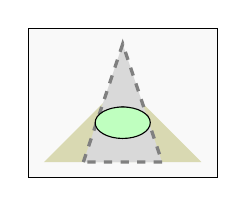
\begin{tikzpicture}
    \draw[fill=gray!5] (0.8,0.8) rectangle (3.2,2.7);
    
    \path[fill=green!50!red!30] (1,1) -- (2,2) -- (3,1) -- cycle; %cycle to connect the points
    
    \path[draw=gray,very thick, style=dashed,fill=gray!30] (1.5,1) -- (2,2.5) -- (2.5,1) -- cycle; %here draw=gray draws the outline of the inside triangle

    \draw[fill=red!25] (2,1.5) circle (0.2);

    \draw[fill=green!25] (2,1.5) ellipse (0.35 and 0.2);    
\end{tikzpicture}\newline


\section{Connecting node like a triangle}
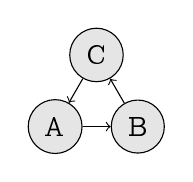
\begin{tikzpicture}[scale=0.7]
    \node[circle,draw,fill=gray!20] (a) at (0,0) {A};
    \node[circle,draw,fill=gray!20] (b) at (0:1.5) {B}; % (angle:distance), here : is used while considering angle
    \node[circle,draw,fill=gray!20] (c) at (60:1.5) {C};
    \draw[->] (a) -- (b);
    \draw[->] (b) -- (c);
    \draw[->] (c) -- (a);   
\end{tikzpicture}\\


\section{Using loop to draw multiple nodes}
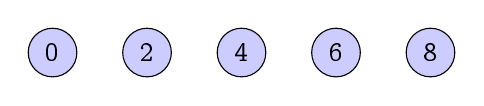
\begin{tikzpicture}[scale=0.6]
    \foreach \n in {0, 2, ..., 9}  \node[circle,draw,fill=blue!20] at (\n,0) {\n};
\end{tikzpicture}\\ 

\section{Connect circular nodes with arrows from centre}
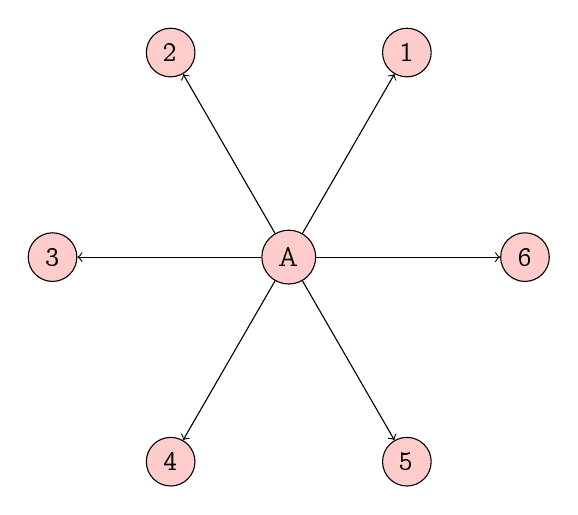
\begin{tikzpicture}
    %central node
    \node[circle,draw,fill=red!20] (a) at (0,0) {A}; 
    \foreach \n in {1, 2, ..., 6} \node[circle,draw,fill=red!20] (\n) at (60*\n:3) {\n};
    \foreach \n in {1, 2, ..., 6} {
        \draw[->] (a) -- (\n); % Arrows from central node (a) to each other node
    }    
\end{tikzpicture}


\section{Connect circular nodes with arrows as a circle}

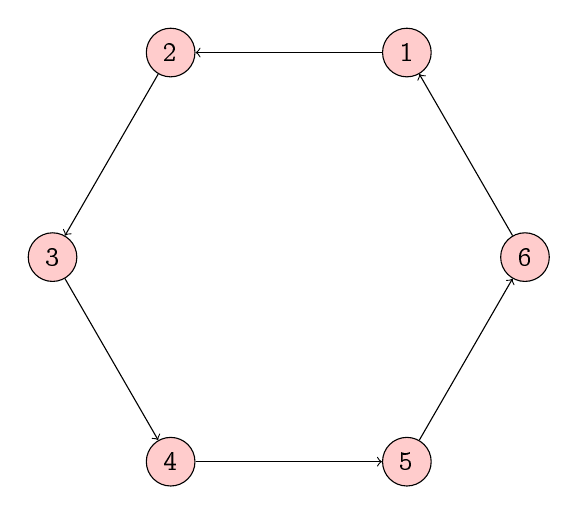
\begin{tikzpicture}
    \foreach \n in {1, 2, ..., 6} \node[circle,draw,fill=red!20] 
    (\n) at (60*\n:3) {\n};
    \foreach \n [count=\next from 2] in {1, 2, ..., 6} {
        \ifnum\n=6
            \break % Fake "break" (prevents further drawing but
            technically still iterates)
        \else
            \draw[->] (\n) -- (\next);
        \fi
    }
    % Manually connect last node back to first
    \draw[->] (6) -- (1);   
 \end{tikzpicture}

 
\subsection{\texttt{LaTeX code:}}
%\begin{tcolorbox}[colback=gray!20,colframe=black!75,boxrule=0.5mm]
%\begin{verbatim}
\begin{lstlisting}[language={[LaTeX]TeX}]
 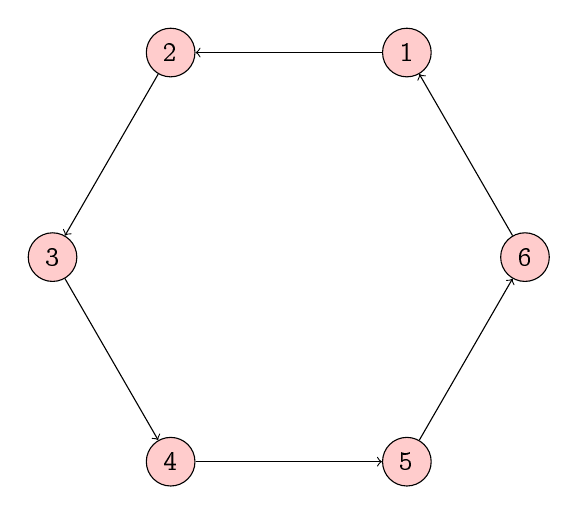
\begin{tikzpicture}
    \foreach \n in {1, 2, ..., 6} \node[circle,draw,fill=red!20]  (\n) at (60*\n:3) {\n};
    \foreach \n [count=\next from 2] in {1, 2, ..., 6} {
        \ifnum\n=6
            \break % Fake "break" (prevents further drawing but technically still iterates)
        \else
            \draw[->] (\n) -- (\next);
        \fi
    }
    % Manually connect last node back to first
    \draw[->] (6) -- (1);   
 \end{tikzpicture}
 \end{lstlisting}
%\end{verbatim}
%\end{tcolorbox}




%\tikz \graph [tree layout, sibling distance=1 cm, nodes={circle, draw},grow=right]
%{ 1--{2--{6,7,8},3--{11,12},4--{13},5--{9,10}} };


\end{document}
